\documentclass[a4paper]{article}
\usepackage[utf8]{inputenc}
\usepackage{graphicx}
\graphicspath{ {imgs/} }
\usepackage{floatrow}
\usepackage{array}
\usepackage[margin=1in]{geometry}
\usepackage{courier}
\usepackage{etoolbox}
\usepackage[htt]{hyphenat}
\usepackage[dvipsnames,table]{xcolor}
\usepackage{listings}
\usepackage{makecell}

\renewcommand\theadalign{bc}
\renewcommand\theadfont{\bfseries}
\renewcommand\theadgape{\Gape[4pt]}
\renewcommand\cellgape{\Gape[4pt]}
\definecolor{codegreen}{rgb}{0,0.6,0}
\definecolor{codegray}{rgb}{0.5,0.5,0.5}
\definecolor{codepurple}{rgb}{0.58,0,0.82}
\definecolor{backcolour}{rgb}{0.95,0.95,0.92}

\lstdefinestyle{mystyle}{
    backgroundcolor=\color{backcolour},   
    commentstyle=\color{codegreen},
    keywordstyle=\color{magenta},
    numberstyle=\tiny\color{codegray},
    stringstyle=\color{codepurple},
    basicstyle=\ttfamily\footnotesize,
    breakatwhitespace=false,         
    breaklines=true,                 
    captionpos=b,                    
    keepspaces=true,                 
    numbers=left,                    
    numbersep=5pt,                  
    showspaces=false,                
    showstringspaces=false,
    showtabs=false,                  
    tabsize=2
}

\lstset{style=mystyle}

\title{\textbf{GIT Department Of Computer Engineering\\ 
CSE 222/505 - Spring 2020\\
Homework 3 Report \vspace{1in}}}

\author{\textbf{Fatih Kaan Salgır} \\ 
\textbf{171044009}}

\date{}

\begin{document}

\begin{large}

  \maketitle

\newpage


\begin{center}
  \textbf{ \\
  \vspace{3cm}
  \Huge{PART 1}
  }
\end{center}

\newpage


\section{Problem Solution Approach}

The assignment is developing an data structure which consist of arrays of nodes. Since it extends \texttt{AbstractList<E>}, I have started to implement methods not implemented in \texttt{AbstractList<E>}. These methods are;

\begin{itemize}
  \item \texttt{void add(int index, E e)}
  \item \texttt{E get(int index)}
  \item \texttt{E remove(int index)}
  \item \texttt{E set(int index, E element)}
  \item \texttt{int size()}
\end{itemize}

All other methods are already inherited or implemented in \texttt{AbstractList<E>} class, or depends on the listed methods.
\vspace{1em}

I separated array to another class since its behavior is different than linked list structure. I made Node class and fields private, because its better practice to encapsulate classes.
\vspace{1em}

I used \texttt{display()} method which is not part of methods I had to implemented it, but I have used this method to debug almost every method, to observe current states of the list structure. It prints total size, size of each node and elements in the nodes. One of its example output is shown below;

\begin{verbatim}
12[3, 1, 2, 8, null]4->[7, 6, 5, 10, 8]5->[9, 3, 2, null, null]3->
\end{verbatim}

Every method with index as parameter has a check mechanism, if given index is in bounds to operate that particular method. I have implemented this control either with \texttt{Objects.checkIndex(index, size)} or \texttt{rangeCheckForAdd(index)}.

\newpage

\section{Class Diagrams}


\begin{figure}[htp]
  \centering
  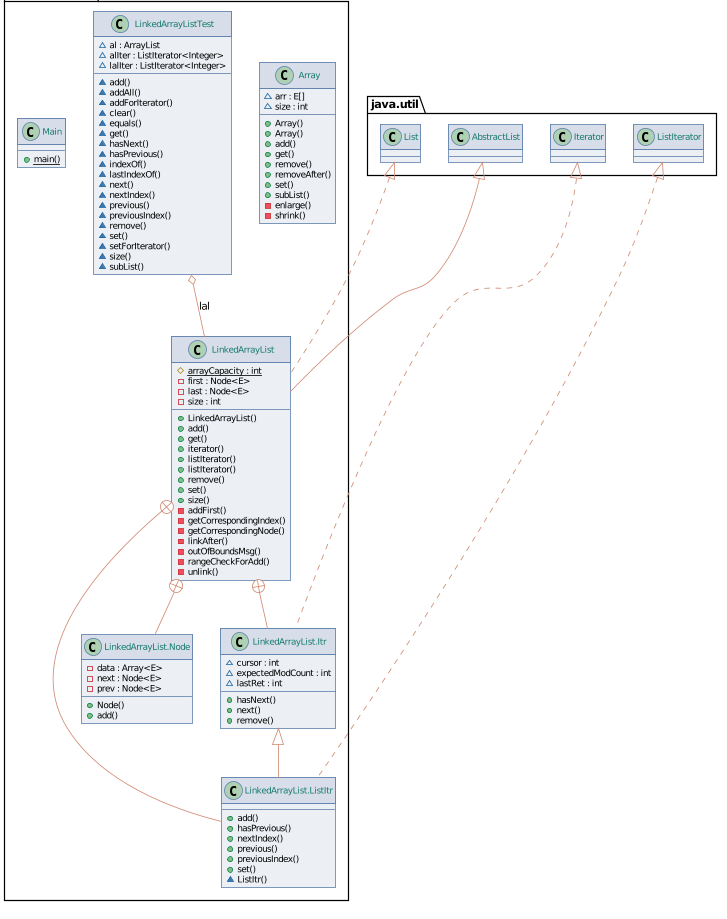
\includegraphics[width=0.95\textwidth]{class-diagram}
\end{figure}

\newpage


\section{Test Cases}

To test all the methods I have created \texttt{LinkedArrayListTest} class which uses JUnit methods. I have created an \texttt{ArrayList} and \texttt{LinkedArrayList} to compare if the list is operates as expected. I called same methods over these two and check them if they are same. After the method calls I used \texttt{assertEquals(lal, al)}.

\begin{lstlisting}[language=Java, caption=Some of the JUnit methods for demonstration]
  @org.junit.jupiter.api.Test void get() {

  void set() {
    add();
    assertEquals(al.set(3, 11), lal.set(3, 11));
    assertEquals(al, lal);
  }

  @org.junit.jupiter.api.Test
  void remove() {
    add();
    assertEquals(al.remove(1), lal.remove(1));
    assertEquals(al.remove(new Integer(3)), lal.remove(new Integer(3)));
  }

  @org.junit.jupiter.api.Test
  void size() {
    add();
    assertEquals(al.size(), lal.size());
    assertEquals(al, lal);
  }
\end{lstlisting}


I have created some text cases for some adding and removing operations which is present on my main method.

\begin{center}
\begin{table}[htp]
  \rowcolors{1}{black!5}{gray!5}
\begin{tabular}{ |m{1cm}|m{3cm}|p{3cm}|m{6em}|m{6em}|m{2cm}|l|  }
 \hline
  \rowcolor{RoyalBlue!30}
 \thead{Test \\ Case \\ ID} & \thead{Test \\ Scenario} & \thead{Test Steps} &\thead{Expected \\ Results} & \thead{Actual \\ Results} & \thead{Pass/Fail}\\
 \hline
 \makecell{T01} & add end of the list & \makecell[l]{1. add(1)\\ 2. add(2)} & \makecell{[1,2]} & \makecell{As expected} & \makecell{Pass}  \\
 \hline
 \makecell{T02} & remove from end of the list & \makecell[l]{1. add(1)\\ 2. add(2)\\3. remove(1)} & \makecell{[1]} & \makecell{As expected} & \makecell{Pass}  \\
 \hline
 \makecell{T03} & add beginning of the list & \makecell[l]{1. add(1)\\ 2. add(0, 2)} & \makecell{[2,1]} & \makecell{As expected} & \makecell{Pass}  \\
 \hline
 \makecell{T04} & add middle of the list & \makecell[l]{1. add(0)\\ 2. add(2) \\ 3. add(1,1)} & \makecell{[0,1,2]} & \makecell{As expected} & \makecell{Pass}  \\
 \hline
 \makecell{T05} & add or remove greater or less than size& \makecell[l]{add(-1,0)\\add(100,0)\\remove(-2)\\remove(100)} & \makecell{Throw \\ exception} & \makecell{As expected} & \makecell{Pass}  \\
 \hline
\end{tabular}

\end{table}

\end{center}

\newpage

\section{Running and Results}

\begin{figure}[htp]
  \centering
  \caption{main - test cases}
  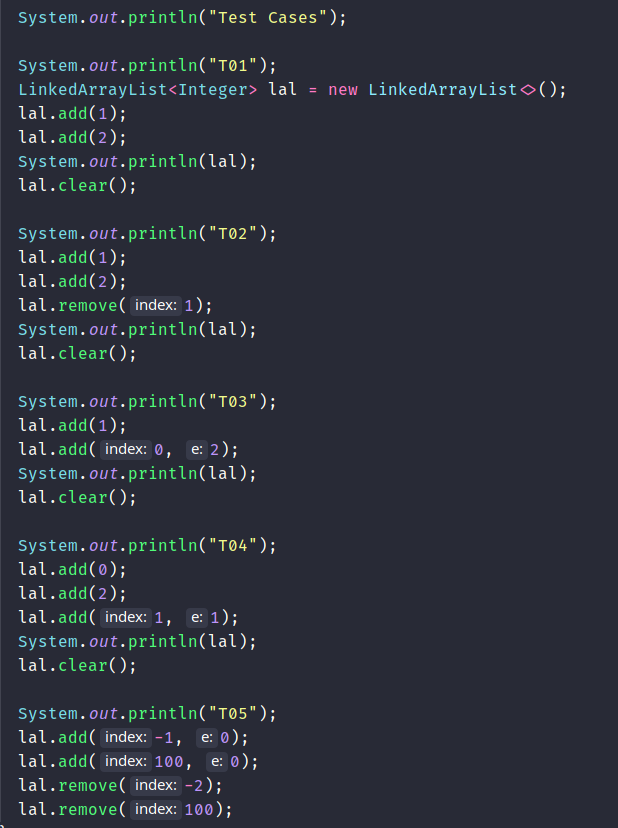
\includegraphics[width=0.55\textwidth]{main-test}
\end{figure}

\begin{figure}[htp]
  \centering
  \caption{Output of main method after tested cases}
  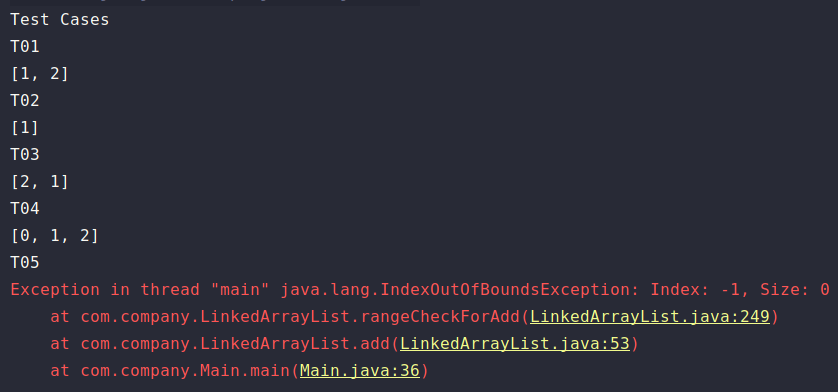
\includegraphics[width=0.7\textwidth]{main-out}
\end{figure}

\newpage

\begin{center}
  \textbf{ \\
  \vspace{3cm}
  \Huge{PART 2}
  }
\end{center}

\newpage

\setcounter{section}{0}

\section{Problem Solution Approach}


The assignment is developing an simple text editor. We supposed to do it by using different lists and different iteration methods. Therefore I decided to separate these methods into different classes. I started by coding and interface since we know basics of text editor. Method calls for lists should be same, so I separated classes by their iteration type. I have preferred to use an \texttt{AbstractList<E>} and use desired list by calling as a constructor parameter.
\vspace{1em}

While I coding classes, I have realized that I needed some common methods for different classes such as; \texttt{readFile(), rangeCheck()} methods. Therefore I have created an abstract class on top of these classes, and put common methods in this abstract class. At the end, I have 2 main classes which are \texttt{TextEditorIterator} and \texttt{TextEditorLoop} according to their way of iteration. I didn't implement replace method 2 times to avoid code repetition. Replace method already calls appropriate find method according to type of the iteration.
\vspace{1em}

In \texttt{TextEditorIterator} class I mostly used enhanced for loop, since it works with iterators.
\vspace{1em}

For testing methods, I used a lorem ipsum file. It consist of 100 paragraphs which is relatively long text so that, I can compare the runtimes of methods more accurately. I thought comparing runtimes as milliseconds would be enough. For measuring runtime and logging, I created a \texttt{Loger} class.
\vspace{1em}

\newpage

\section{Class Diagrams}

\begin{figure}[htp]
  \centering
  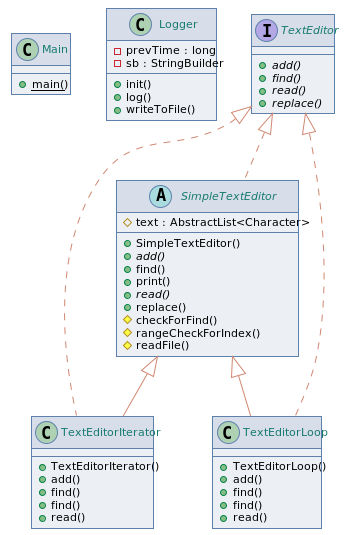
\includegraphics[width=0.6\textwidth]{class-diagram-2}
\end{figure}

\newpage

\section{Test Cases}

To test all the methods I called methods with same parameters for different types of lists and different types of iteration. Between these calls I called \texttt{log()} method to measure runtime of methods. 
\vspace{1em}

I have created some text cases for operations. They are present on my main method.


\begin{center}

  \begin{table}[htp]
  \rowcolors{1}{black!5}{gray!5}
    
\begin{tabular}{ |m{2em}|m{3cm}|p{8em}|m{6em}|m{6em}|m{2cm}|l|  }
 \hline
  \rowcolor{RoyalBlue!30}
 \thead{Test \\ Case \\ ID} & \thead{Test \\ Scenario} & \thead{Test Steps} &\thead{Expected \\ Results} & \thead{Actual \\ Results} & \thead{Pass/Fail}\\
 \hline
 \makecell{T01} & find & \makecell[l]{find(``libero(f)")} & \makecell{32611} & \makecell{As expected} & \makecell{Pass}  \\
 \hline
 \makecell{T02} & add text at the beginning of the file& \makecell[l]{add(0,"deneme")} & {return 1, adds begining of the list} & \makecell{As expected} & \makecell{Pass}  \\
 \hline
 \makecell{T03} & add text in the middle of the list & \makecell[l]{add(32611, ****")} & adds position 32611, return 1 & \makecell{As expected} & \makecell{Pass}  \\
 \hline
 \makecell{T04} & replace & \makecell[l]{replace(`o',`\_')} & \makecell{2281 \\ repalce chars} & \makecell{As expected} & \makecell{Pass}  \\
 \hline
 \makecell{T05} & replace nonexistent char & \makecell[l]{replace(`8',`a')} & \makecell{0} & \makecell{As expected} & \makecell{Pass}  \\
 \hline
 \makecell{T06} & find nonexistent char & \makecell[l]{find(``asdf")} & \makecell{-1} & \makecell{As expected} & \makecell{Pass}  \\
 \hline
 \makecell{T07} & calling methods greater or less than size& \makecell[l]{add(-1,``x")\\add(999999, ``x")} & \makecell{Throw \\ exception} & \makecell{As expected} & \makecell{Pass}  \\
 \hline
\end{tabular}
  \end{table}

\end{center}

\begin{lstlisting}[language=Java]
System.out.println("Test Cases");
iterAL.add(0, "deneme");
loopAL.add(0, "deneme");
System.out.println(iterAL.replace('8', 'a'));
System.out.println(iterAL.find("asdf"));
System.out.println(loopAL.replace('8', 'a'));
System.out.println(loopAL.find("asdf"));
iterAL.add(-1, "x");
iterAL.add(999999, "x");

\end{lstlisting}

\begin{small}
\begin{verbatim}
String found at: 32611
2281 replaced chars.
String added specified position.
**ArrayList and iterator is used**
String found at: 32611
2281 replaced chars.
String added specified position.
**LinkedList and loop is used**
String found at: 32611
2281 replaced chars.
String added specified position.
**ArrayList and loop is used**
String found at: 32611
2281 replaced chars.
String added specified position.
\end{verbatim}
\end{small}

\newpage

\section{Running and Results}

\subsection{Theoretic Analysis}

\subsection*{ArrayList - Iterator}
\begin{itemize}
  \item \texttt{read}: $\theta(n)$
  \item \texttt{add}: $\theta(1)$, as long as there is enough space in the array. $\theta(n)$ otherwise.
  \item \texttt{find}: $O(n)$
  \item \texttt{replace}: $O(n)$
\end{itemize}

\subsection*{ArrayList - Loop}
\begin{itemize}
  \item \texttt{read}: $\theta(n)$
  \item \texttt{add}: $\theta(1)$, as long as there is enough space in the array. $\theta(n)$ otherwise.
  \item \texttt{find}: $O(n)$
  \item \texttt{replace}: $O(n)$
\end{itemize}

\subsection*{LinkedList - Iterator}
\begin{itemize}
  \item \texttt{read}: $\theta(n)$
  \item \texttt{add}: $O(n)$
  \item \texttt{find}: $O(n^2)$
  \item \texttt{replace}: $O(n^2)$
\end{itemize}

\subsection*{LinkedList - Loop}
\begin{itemize}
  \item \texttt{read}: $\theta(n)$
  \item \texttt{add}: $O(n)$
  \item \texttt{find}: $O(n^2)$
  \item \texttt{replace}: $O(n^2)$
\end{itemize}

\newpage

\subsection{Analysis of runtimes}

\texttt{read} method is almost same, it has the same complexity for all of them.
\vspace{1em}

\texttt{add} method for \texttt{ArrayList} is constant time, it is `$< 1ms$' both with iterator and loop. Since \texttt{get} methods works in constant time. In \texttt{LinkedList} although it has the complexity of $O(n)$ still pretty fast to iterate through nodes. Therefore the differnce between runtimes is not observable.
\vspace{1em}

\texttt{find, replace}: Main reason of getting such a long runtimes for \texttt{LinkedList} is initalizing \texttt{ListIterator} with an index. Every time second iterator is initalized in find method, it has to iterate to specific position from beginning.
\vspace{1em}

Since we don't use remove and add extensively, we don't make use of benefits of linked list.
\vspace{1em}

\begin{lstlisting}[caption=Log file]
Running Time (ms)     Message
           19 ms:     read method, LinkedList with Iterator
          812 ms:     find method, LinkedList with Iterator
         1476 ms:     replace method, LinkedList with Iterator
            0 ms:     add method, LinkedList with Iterator
            5 ms:     read method, ArrayList with Iterator
            6 ms:     find method, ArrayList with Iterator
            7 ms:     replace method, ArrayList with Iterator
            0 ms:     add method, ArrayList with Iterator
            6 ms:     read method, LinkedList with loop
          732 ms:     find method, LinkedList with loop
         1465 ms:     replace method, LinkedList with loop
            0 ms:     add method, LinkedList with loop
            3 ms:     read method, ArrayList with loop
            4 ms:     find method, ArrayList with loop
            2 ms:     replace method, ArrayList with loop
            0 ms:     add method, ArrayList with loop
\end{lstlisting}

\newpage

\begin{center}
  \textbf{ \\
  \vspace{3cm}
  \Huge{PART 3}
  }
\end{center}

\newpage

\setcounter{section}{0}

\section{Problem Solution Approach}

I started by creating a \texttt{Node} class which stores a character, both next and previous references to other character and cross node if there is any. While implementing \texttt{public} methods I added error handling methods. These methods are \texttt{checkCrossesAreSameChar(..)} which checks while adding a cross word if the characters are the same and \texttt{checkIndex(..)} which checks if indexes are in bounds. Both of these methods throws exception in necessary conditions.
\vspace{1em}

In \texttt{CrossWordPuzzle} there are two adding and two removing operation. The difference between them is; while one of them is adding with all of its cross words other is only adds that word.
\vspace{1em}

To test methods, I build the same puzzle in the assignment, added words with its cross words. Then I tested with another custom puzzle.


\newpage

\section{Class Diagrams}

\vspace{1em}

\begin{figure}[htp]
  \centering
  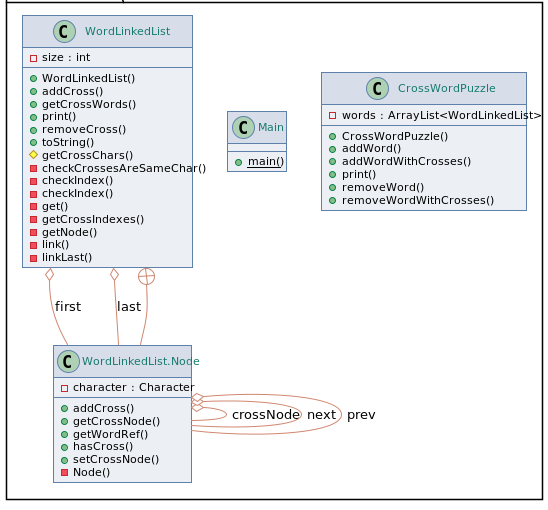
\includegraphics[width=\textwidth]{class-diagram-3}
\end{figure}

\newpage

\section{Test Cases, Running and Results}

Along with the demonstration in the assignment custom test case I used;

\begin{figure}[htp]
  \centering
  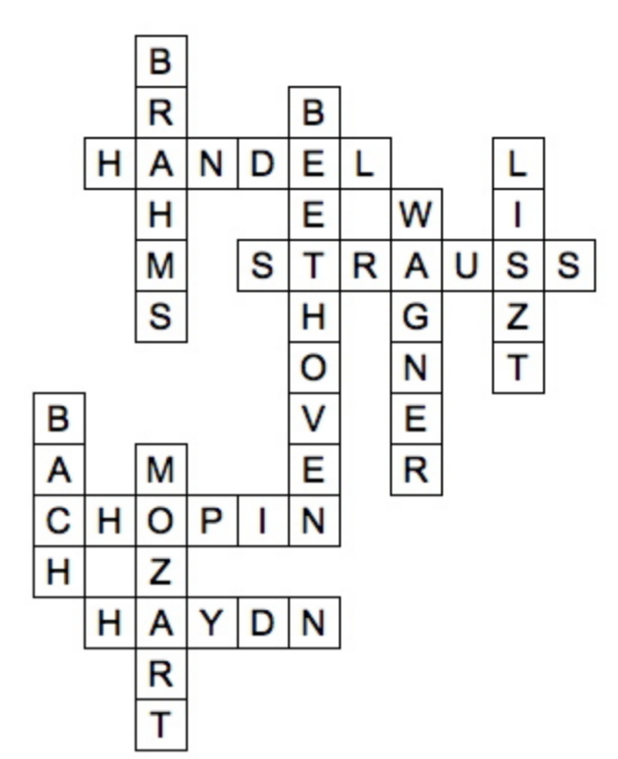
\includegraphics[width=0.4\textwidth]{crossword}
\end{figure}


\begin{lstlisting}[caption=Main output]
**ADD TEST**
PUZZLES: { 1:FUN 6:CROSSWORD }
FUN: { 1:PUZZLES }
CROSSWORD: { 1:ARE 4:PUZZLES }
ARE: { 1:CROSSWORD }

**REMOVE TEST**
FUN removed
PUZZLES: { 6:CROSSWORD }
CROSSWORD: { 1:ARE 4:PUZZLES }
ARE: { 1:CROSSWORD }

**SECOND PUZZLE**
BRAHMS: { 2:HANDEL }
HANDEL: { 1:BRAHMS 4:BEETHOVEN }
BEETHOVEN: { 1:HANDEL 3:STRAUSS 8:CHOPIN }
STRAUSS: { 1:BEETHOVEN 3:WAGNER 5:LISZT }
CHOPIN: { 0:BACH 2:MOZART 5:BEETHOVEN }
WAGNER: { 1:STRAUSS }
LISZT: { 2:STRAUSS }
BACH: { 2:CHOPIN }
MOZART: { 1:CHOPIN 3:HAYDN }
HAYDN: { 1:MOZART }
\end{lstlisting}

\end{large}
\end{document}

